% !TEX root = ../thesis-example.tex
%
\chapter{Related Work}
\label{chapter2}

\cleanchapterquote{An iPod, a phone, an internet mobile communicator... these are NOT three separate devices! And we are calling it iPhone! Today Apple is going to reinvent the phone. And here it is.}{Steve Jobs}{MacWorld 2007}

\section{Native applications}
Native apps are applications built for particular platforms. These applications are written in Java, Dart or Kotlin for Android, and Swift or Objective-C for iOS. Regarding native applications, automated mobile app testing has been explored profusely in many areas (\eg frameworks, automation APIs, testing techniques, GUI exploration, security, usability, error reporting tools)\cite{linares-vasquez_moran_poshyvanyk_2017}, \cite{zein_salleh_grundy_2016}, \cite{Choudhary:ASE15}, \cite{Kochhar:ICST15}. In this section we focus specifically on two aspects: testing frameworks and GUI ripping tools (due to the nature of model extraction based on GUI events), which are closer to our proposal.
\subsection{Testing frameworks}

Frameworks for mobile testing define principles, concepts and architectures to structure testing processes. To this end,  one of the frameworks where automated extraction of augmented models have been explicitly defined is CEL \cite{linares-vasquez_moran_poshyvanyk_2017}. CEL is based on three main principles: \emph{continuous}, \emph{evolutionary} and \emph{large-scale}. The first principle, \emph{continuous}, refers to the fact that mobile apps should be tested under multiple environmental conditions and according to different goals. The second principle, \emph{evolutionary}, sets forth that testing artifacts like the models, should adapt to changes in source code, environment, and in-the-wild usages. Lastly, the \emph{large-scale} principle proposes an engine to execute test cases in real and emulated devices to tackle fragmentation.

With this in mind, the CEL framework argues that there must be a ``models generator'' component that combines multiple models such as GUI, usage, and contextual models to finally create a multi-model representation of an app under test. This multi-model can be used for the evolutionary generation of testing artifacts \cite{linares-vasquez_moran_poshyvanyk_2017}. CEL affirms that current approaches for deriving  representations of apps are severely lacking a multi-model-based approach that might significantly improve the utility of model-based testing \cite{linares-vasquez_moran_poshyvanyk_2017}. Having said that, our approach of extraction of an augmented model fits CEL's principles and architecture, enhancing GUI exploration with complementary models. Note that the CEL paper does not provide any detail regarding how a multi-model should be; thus, we are the first to instantiate the multi-model concept as proposed by CEL.

\subsection{GUI ripping tools}
\label{native:ripping}
GUI ripping tools  simulate real user events on an Android device to explore an application GUI. The majority of these tools detect and report crashes generated during the exploration. Coupled with detection of crashes, others of these tools also reconstruct GUI models resulting from the exploration (\eg MonkeyLab \cite{monkeylab}, AimDroid\cite{aimDroid}, Android Ripper \cite{amalfitano_fasolino_tramontana_carmine_memon_2012}). Previous effort has been also focused on tools that build testing suites based on their exploration strategy (\eg Sapienz \cite{mao_harman_jia_2016}, MobiGUITAR \cite{amalfitano_fasolino_tramontana_ta_memon_2015}).

DroidBot\cite{Li:ICSE17} is another tool that uses a model-based strategy to automatically explore mobile GUI based on a DFS effective strategy. It generates inputs and a transition model between different states of the application. One of the main features of DroidBot is that it does not require app instrumentation and is mean to run in almost any Android device.

Firebase Test Lab \cite{firebase} is one of the industry leaders in mobile testing. It has a cloud-based app-testing infrastructure that enables concurrent execution of tests with and without instrumentation. Firebase Test Lab Robo Test is one of their services: 'Robo test analyzes the structure of your app's UI and then explores it methodically, automatically simulating user activities' \cite{firebase}. It cloud service allows testers to run Robo test on virtual and physical devices in parallel, detecting crashes and performance issues. 

The aforementioned tools have advanced significantly in terms of algorithms to explore apps' GUI. They systematically create state diagrams based on GUI information and GUI states exploration. However, GUI ripping tools lack information about the execution context that could help to determine contextual states, \eg a navigation app without GPS and Internet can not be as functional as it was intended to be, because turning GPS on and off in the same activity could result into two totally different states. GUI rippers also lack information about domain and usage of the application. However, effective mobile testing requires considering different types of information (\ie GUI, domain entities, contextual states, real usages) because combining more information could drive to exploring more states in an app.

As mentioned before, there are tools that reconstruct GUI models resulting from ripping and simulated user interactions. These approaches try to generate sequences of events under a particular strategy that drives and explores apps. \cite{aimDroid}. Most of these tools generate finite-state machines with two purposes: (i) there is a need to generate sources of information to understand a system, whose models are nonexistent or too precarious. \cite{7516816}; and (ii)  model-based testing requires models to automate model generation processes.

Other approximations such as CrashScope \cite{crashscope} systematically explores Android apps and creates detailed crash reports in natural language. CrashScope enables context-aware input data and sensors and connectivity analysis. CrashScope makes contextual changes in the application based on API calls found statically in the code. 

\textit{Contextual fuzzing} is also an approach implemented in \textit{Caippa}~\cite{Liang:MobiCom14}, a service for testing Windows mobile apps in a cloud environment. Contextual fuzzing refers to exercising apps with contexts observed in the wild (\eg eventual connectivity). In this case, GUI ripping is performed along the contextual fuzzing.

Injection of adverse conditions have been also explored not only with GUI ripping, but also using existing test cases. This is the case of \textit{Thor} \cite{Adamsen:ISSTA2015}, a tool that injects unexpected events (\ie device rotation or incoming calls) in existing test suites.

%, however, it lacks generation of contextual changes that were not previously coded in the app. 

%There are other approximations different that ripping, that generate models from usage scenarios manually recorded by testers. After interactions have been recorded, actionable scenarios are  automatically replicated and transformed to generate streams of events. \cite{crashscope}.

%Above all, the need to capture more than GUI information prevails, in order to have better understanding of software, specifically, Android mobile apps.
Above all, previous research have used GUI models  \cite{monkeylab}, \cite{aimDroid}; combined usage  and GUI models \cite{mao_harman_jia_2016}, \cite{amalfitano_fasolino_tramontana_ta_memon_2015}, \cite{Li:ICSE17}; GUI and context models (partially)  \cite{crashscope}, \cite{Liang:MobiCom14}; and context information with existing tests \cite{Adamsen:ISSTA2015}. However, none of the aforementioned approached have covered the multi-model vision we are proposing.

\section{Hybrid applications}

Hybrid apps are those in which developers write significant portions of their application in cross-platform web technologies, while maintaining direct access to native APIs when required \cite{ibmHybrid}. This way of developing applications is gaining popularity among the mobile developers community because:
\begin{itemize}
	\item Reduces the time to develop cross-platform apps
	\item It is based on Web technologies, which allows developers to recycle modules and components from existing Web developments
	\item Browser engines are becoming faster and mobile devices more powerful
	\item Performance differences between native and web technologies are becoming imperceptible
\end{itemize}
The industry leaders in hybrid applications are \textit{React Native} and \textit{Apache Cordova}, two different approximations with fundamental differences.
\subsection{React Native}
React native is a Facebook project that enables the construction of mobile apps based on React: a Javascript library. In this case, the code written in JS runs in a thread and do not cross-compile to other languages. To manage the GUI, React native uses the Android GUI framework, which means that graphical elements from an application built using this technology should be indistinguishable from the graphical components of a native application. 

Given the fact that crawling and ripping Android applications is done through examination of the native graphical components, this kind of apps could be ripped used the existing GUI ripping tools aforementioned.

\subsection{Apache Cordova}
Apache Cordova is another technology that enables the access to native APIs from JS code. This piece of software gives access to Local Storage, Camera, GPS, and all the available sensors of each platform. Apache Cordova is the core of many popular hybrid frameworks such as Ionic, Adobe Phonegap, Monaca or Visual Studio. 

The main difference from Apache Cordova to React Native is related to the way the GUI components are presented to the user. Contrary to React Native, Apache Cordova does not use native components. This technology encapsulates a Web Application based on JS, HTML and CSS into a Web View. Fig \ref{hybridCordova}.

\begin{figure}[t]
	\centering
	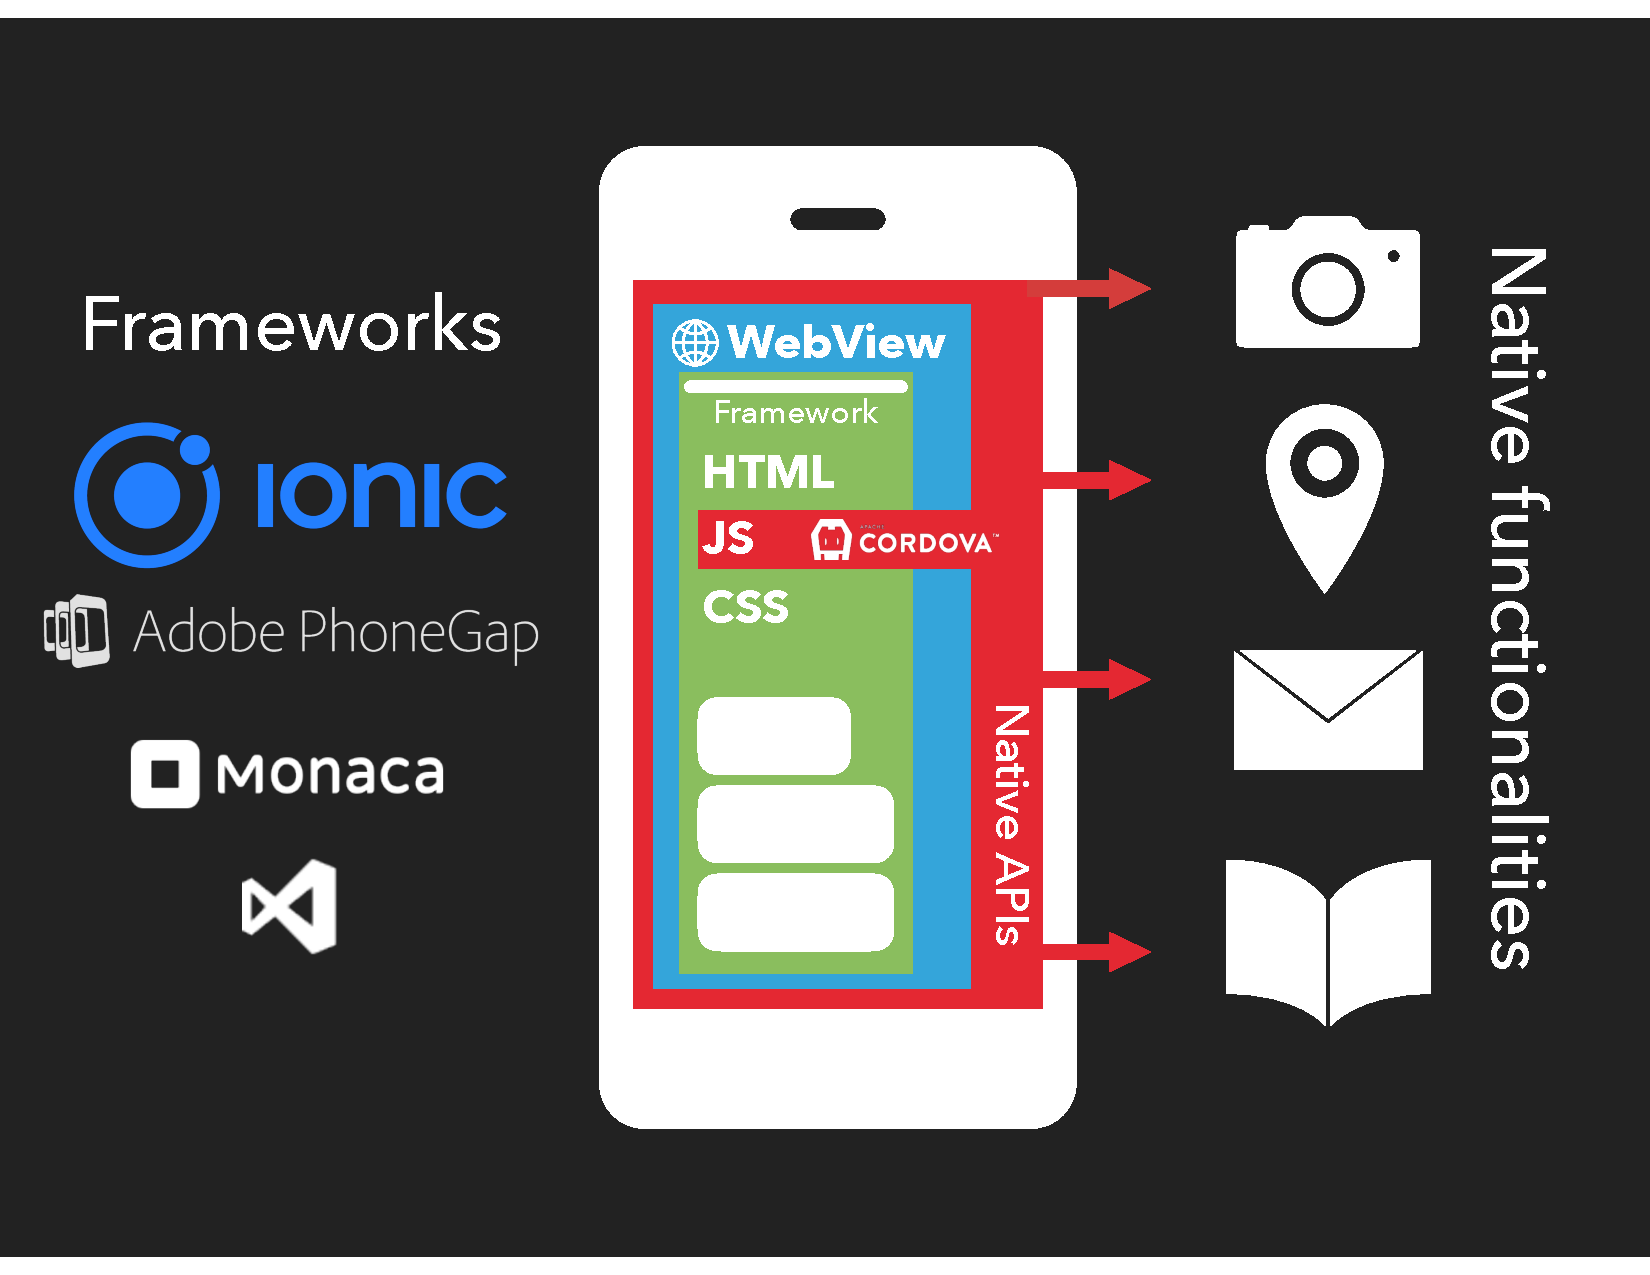
\includegraphics[width=1\textwidth]{img/hybrid.pdf}
	\vspace{-0.8cm}
	\caption{Contrary to native applications, Apache Cordova based applications contain just one activity. This activity has a basic layout with a central element: a \textit{Web view}}
	\label{hybridCordova}
\end{figure} 


Because of the differences between React Native and Apache Cordova, some argument that React Native is not hybrid. Given the fact that React Native apps can be crawled as native applications, henceforth, when we refer to hybrid applications we will refer exclusively to apps that use a Web View to present the GUI.

\subsection{Testing  hybrid applications}

Most of the research conducted in hybrid applications is focused in two categories: Debugging and Security.

\subsubsection{Debugging}

The most popular tool for debugging hybrid applications and remote web views is Chrome Developer Tools \cite{cdt}. These tools are directly built into the Google Chrome browser. Accessing to \texttt{chrome://inspect} displays the lists of web views in the devices connected through ADB. Once the browser is remotely inspecting the web view, all the errors, crashes and logs from JavaScript are printed in the computer's console. With Google Chrome, developers have access in real time to the DOM elements, network settings, and JS console to profile and audit the applications performance.

The first remote debugger was introduced in 2010: winre (WEb INspector REmote)\cite{weinre}. It was part of the Apache Cordova project, however it is being deprecated due to the increasing functionality of the Google Developer Tools. There are tools based on Google Developer Tools that enhance debugging functionality, such as the Monaca Debugger\cite{monacaDebugger} which include Cordova Plugins Supoprt and collaboration tools.


There is an approach to debug hybrid applications based on static analysis: HybriDroid\cite{7582763}.  It includes a built in bug detector based on a call graph which founds 4 types of bugs: MethodNotFound (when a JavaScript method call cannot find any target Java method to call), TypeOverloadedBridgeMethod (when JavaScript tries to use Java overloading), NotCompatibleTypeConversion (when a JavaScript type is not compatible with Java), and MethodNotExecuted (when a Java method returns an Array)\cite{7582763}.

\subsubsection{Security}

Tools and techniques related to security, are relevant to our approach because they examine the web view, and are able to analyze properties of hybrid applications.

This has been an important research topic in hybrid applications because of the possibilities of \textit{cross-language code injection}. Jin \textit{et al.} \cite{Jin:2014:CIA:2660267.2660275} define that this problem is inherited from Cross-Site scripting (XSS); additionally to their study, they developed a vulnerability detection tool.  These vulnerabilities have been detected, and numerous tools to report them have been created: NOFRAK \cite{georgiev_jana_shmatikov_2014}, Draco \cite{Tuncay:2016:DSU:2976749.2978322}, \cite{10.1007/978-3-319-27659-5_22}. Some of these approaches are based on instrumentation to  reduce the attack surface \cite{Shehab:2014:RAS:2688412.2688417}. BridgeTaint\cite{8410576} is 'a bi-directional dynamic taint tracking method that
can detect bridge security issues in hybrid apps' \cite{8410576}. It analyzes privacy leaks and code injection when the app uses bridge communication dynamically. Another tool that addresses this problem is HybriDroid\cite{7582763} which additionally to the bug detector, detects taints and leaks between Java and JavaScript. In comparison, BridgeTaint is able to detect security issues of apps built with frameworks, when HybriDroid sometimes do not.

Another topic related to security is the detection of SSL errors, Zuo  \textit{et al.} \cite{Zuo:2015:ADS:2714576.2714583} present an approach to detect statically and dynamically vulnerabilities of this kind.

\subsubsection{GUI ripping tools}

As described above, GUI ripping tools for native apps are diverse and numerous, however, as of today, there is not a single approach that focuses on GUI ripping or crawling based on hybrid applications (based on a web view). Some of the tools mentioned in section \ref{native:ripping} could work because of their implementation and the dynamic detection of components, nevertheless, they have flaws detecting different states and crashes.



